\section{Feature Learning}
We now take a re-look at the NTF and NTK matrices, and explicitly write down the terms related to feature learning. \hfill\\
\textbf{ReLU artefact:} Recall that the neural tangent feature is given by $\psi_{x,t}=\phi^\top_{x,t} {\partial} v_t + {\partial} \phi^\top_{x,t} v_t$. We note that, in the case when $A_t(x,p)\in\{0,1\}$ (such as in DNN with ReLU activations)  $\partial_{\phi}=0$, and hence is not accounted for in the SGD update as well as in the trajectory analysis. However, due to the SGD update, the gating value changes during training, and consequently the activations, the NPF, the NPK change during training as seen in the experiments in \Cref{sec:generalisation}. We side step this artefact by studying network with soft-gates: given a pre-activation input, a hard gate (uch as ReLU) uses $\mathbbm{1}_{\{q>0\}}$, while a soft-gate uses a soft-max sigmoidal function $\chi_\epsilon(q)=\frac{1+\epsilon}{1+\exp(-\beta q)}$.\hfill\\ %We consider sofr-ReLU networks denoted by $\N_{SR}(\Theta_t)$, and soft-GaLU networks denoted by $\N_{G}(\Theta_t, \G(\N_{SR}(\Tg_t)))$. %We checked the performance of soft-gates by training, a soft-GaLU network and a soft-ReLU network, and the fact that adaptable gates generalise better than frozen gates continued to hold (see \Cref{fig:gen} which shows the performance of all the $4$ networks namely ReLU, frozen-GaLU, soft-GaLU and soft-ReLU).
\textbf{NTK and feature learning:} For the sake of simplicity we study the case of  soft-GaLU networks, wherein, there are two set of parameters (total $2d_{net}$). Here, the neural tangent feature is given by $\psi_{x,t}=[\psi^v_{x,t},\psi^a_{x,t}]=[\partial_{\Theta} \hat{y}_t, \partial_{\Tg} \hat{y}_t]\in \R^{2d_{net}}$. Thus the NTK matrix is given by $K_t=K^w_t+K^a_t$,  where $K^w_t={\Psi^v_t}^\top \Psi^v_t$, and $K^a_t={\Psi^a_t}^\top \Psi^a_t$, with $\Psi^v_t=[\psi^v_{x_s,t},s\in[n]]$ and $\Psi^v_t=[\psi^a_{x_s,t},s\in[n]]$ are the NTF matices. In the case of  soft-ReLU networks, i.e, $\N_{SR}(\Theta_t)$  it is easy to check that $K_t={K^v_t}+{K^a_t}+{\Psi^v_t}^\top {\Psi^a_t}+{\Psi^a_t}^\top {\Psi^v_t}$.
\begin{definition}\label{def:delta}
For a soft-GaLU networks, using any $i\in[d_{in}]$, define $\delta_t(s,s')\stackrel{def}= \underset{{p\rsa i}}{\sum} \sum_{\tg\in\Tg}\frac{\partial A_{t}(x_s,p)}{\partial \tg} \frac{\partial A_{t}(x_{s'},p)}{\partial \tg}$.
\end{definition}
\begin{lemma} Under \Cref{assmp:main}, in soft-GaLU networks we have: (i) $\E{K_0}=\E{K^w_0}+\E{K^a_0}$, 
 (ii) $\E{K^w_0}=\sigma^{2(d-1)} (x^\top x)\odot \lambda_0$,  (iii) $\E{K^a_0}=\sigma^{2d}  (x^\top x)\odot \delta_0$
\end{lemma}
\textbf{Discussion}: \hfill\\
$1.$ Note that in \Cref{def:delta}, $\delta_t$ contains $\partial A_t(x,p)$ terms as opposed to $A_t(x,p)$ term in $\lambda_t$ defined in \Cref{def:lambda}. For a path $p$, if a path contains gates that are very close to either $0$ or $1$, then $\partial A_t(x,p)$ will be very small. Since $\frac{\partial A_{t}(x_s,p)}{\partial \tg}= \sum_{l=1}^{d-1} \Big(\frac{\partial G_{x_s,\Tg_t}(l,\I_l(p))}{\partial \tg} \Big)\Big(\Pi_{l'\neq l} G_{x_s,\Tg_t}(l',I_{l'}(p))\Big)$, for a path $p$ containing $d-1$ gates close to $1$, and only one gate whose pre-activation input is close to $0$ will have a significant $\partial A_t(x,p)$. \hfill\\
$2.$ Let us take the case of classification with cross-entropy loss. Say we have trained till some $T$ epochs with good classification (say close to $100\%$) accuracy. Considering the fact that $\hat{y}_T=\Phi_{\Tg_T}v_{\Theta_T}$, the gradient with respect to $\Tg$ will change the NPF matrix $\Phi_{\Tg_T}$ in such a manner to reduce the loss, i.e., increase the margin of each of the classified examples. We test this hypothesis  of \emph{margin-increase} due to feature learning in the following toy experiment.\hfill\\
\textbf{A Toy Experiment:} We look at a simple neural network with $d_{in}=2$, $w=2$ and $1$-hidden layer (see first diagram on the left in \Cref{fig:feat}). The first layer weights is an identity matrix, and for input $x\in\R^2$ to the network, the first layer output is given by $z_{t}(i)=x(i)G_t(i),i=1,2$, where $G_t(i)=\frac{1}{1+\exp(-\tg(i))},i=1,2$. In this network, there are $2$ paths, and the NPF is given by $\phi_{x,t}=(x(1)G_t(1),x(2)G_t(2))\in \R^2$ (note that this mimics the general structure of the NPF as presented in \Cref{sec:expressivity}).
We check the performance of frozen-gates versus adaptable gates in this network. The dataset is $(x_s,y_s)_{s=1}^{n},n=1000$, wherein, for $s=,1,\ldots,500$, $x_s(1)\stackrel{iid}\sim U[0.1,1]$, and $x_s(2)\stackrel{iid}\sim U[-100,100]$, and $y_s=1$, and for $s=501,\ldots,1000$, $x_s(1)\stackrel{iid}\sim U[-0.1,-1]$, and $x_s(2)\stackrel{iid}\sim U[-100,100]$, and $y_s=-1$. We use the loss function $L_t=\frac{1}{n}\sum_{s=1}^n\frac{1}{1+exp(-y_s\hat{y}_t(x_s))}$. The maximum margin classifier in this case is: predict $+1$ if $x(1)>0$ and else predict $-1$. We trained the simple neural network using gradient descent with step-size of $0.1$, and initialisation $\Tg_0=\Theta_0=(0,0)\in\R^2$ for the following two cases: i) frozen-gates, wherein, we set $\Tg_0=\Tg_t=\Tg_0,\forall t\geq 0$, so that the input features are not transformed, and train only $\Theta_t$ ii) adaptable gates, wherein, we train both $\Tg_t$ and $\Theta_t$. While both cases train for $T=10^4$ epochs, for $T=10^3$ epochs only the model with adaptable gates trains successfully. The results are shown in \Cref{fig:feat}, notice that the right most plot shows that in the case when the gates are adapting, they learn to suppress the second co-ordinate (the scale of $\phi_{x_s,T}$ is from $-15$ to $15$ as opposed to $-100$ to $100$ in $x_s$).
\FloatBarrier
\begin{figure}[h]
\resizebox{\textwidth}{!}{
\begin{tabular}{cccc}
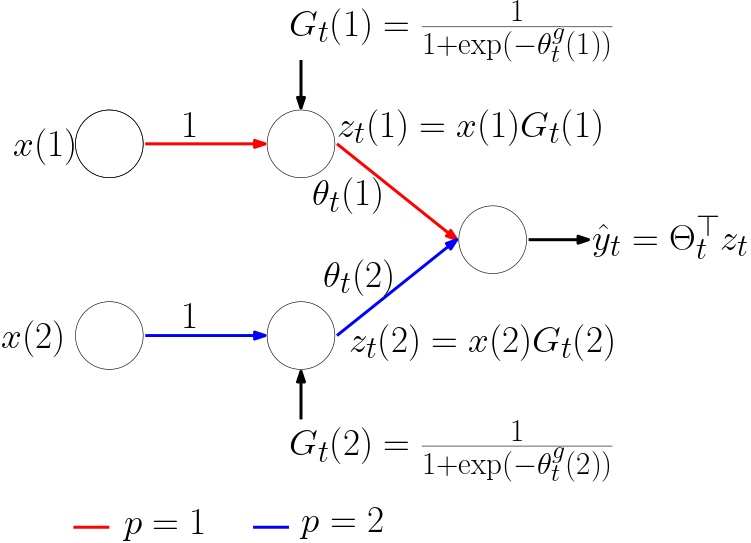
\includegraphics[scale=0.1]{figs/featlearn.png}
&
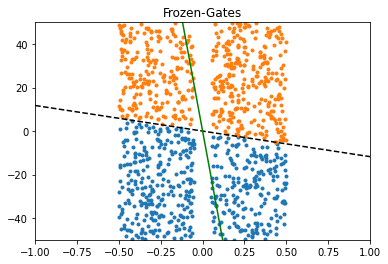
\includegraphics[scale=0.2]{figs/simple.png}
&
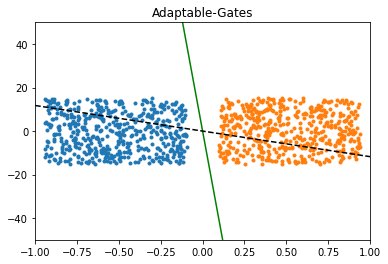
\includegraphics[scale=0.2]{figs/adapt.png}
\end{tabular}
}
\caption{From left: second and third plots shows the training performance of frozen and adaptable gates respectively. In both plots, the bold line in green is the classifier learnt in the case of adaptable gates, and the dotted black line is the classifier learnt in the case of frozen gates. Notice the transformation of the feature space in the case of adaptable gates.}
\label{fig:feat}
\end{figure}
$3.$ \textbf{An open question:} Informally speaking, in the above example, even though the gating parameters had $2$-degrees of freedom, it was nonetheless sufficient to adapt the features. Thus, perhaps we can hypothesise that subject to the `well-conditioned' ness of $K^a_t$, such margin increase can be perhaps achieved for all the $n$ examples.  However, in practice, both $\Tg_t$ as well as $\Theta_t$ change, and an open question is to understand how the joint optimisation and feature learning happens. 